\documentclass[border=10pt]{standalone}
\usepackage{tikz}
\usetikzlibrary{arrows.meta, shapes, calc}

\begin{document}
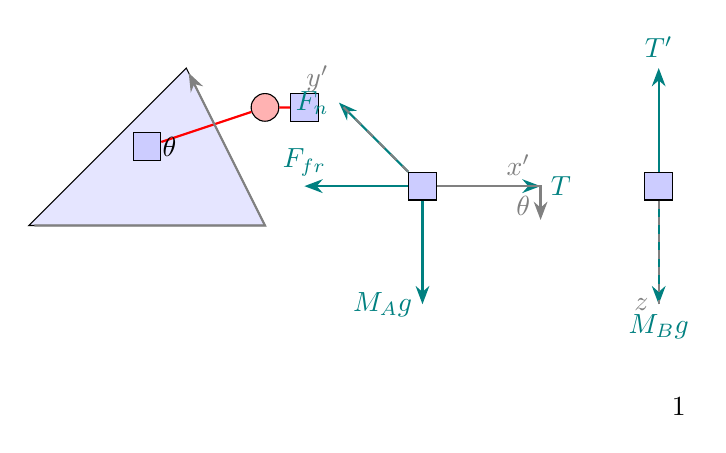
\begin{tikzpicture}[
    block/.style={draw, fill=blue!20, minimum size=10pt, inner sep=2pt},
    pulley/.style={draw, circle, fill=red!30, minimum size=10pt, inner sep=2pt},
    rope/.style={thick, red},
    force/.style={->, >=Stealth, thick, teal},
    axis/.style={dashed, thick, gray},
    angle/.style={->, >=Stealth, thick, gray, shorten <=2pt, shorten >=2pt},
]

% Physical setup (left)
\begin{scope}[shift={(0,0)}]
    % Incline
    \draw[fill=blue!10] (0,0) -- (3,0) -- (2,2) -- cycle;
    % Block A
    \node[block] (A) at (1.5,1) {};
    % Pulley
    \node[pulley] (P) at (3,1.5) {};
    % Block B
    \node[block] (B) at (3.5,1.5) {};
    % Rope
    \draw[rope] (A) -- (P) -- (B);
    % Angle
    \draw[angle] (0,0) -- (3,0) -- (2,2);
    \node[anchor=east] at (2,1) {$\theta$};
\end{scope}

% Free-body diagram for block A (center)
\begin{scope}[shift={(5,0.5)}]
    % Block A
    \node[block] (A) at (0,0) {};
    % Forces
    \draw[force] (A) -- ++(135:1.5) node[anchor=east] {$F_n$};
    \draw[force] (A) -- ++(180:1.5) node[anchor=south] {$F_{fr}$};
    \draw[force] (A) -- ++(0:1.5) node[anchor=west] {$T$};
    \draw[force] (A) -- ++(-90:1.5) node[anchor=east] {$M_A g$};
    % Coordinate system
    \draw[axis] (A) -- ++(135:1.5) node[anchor=south east] {$y'$};
    \draw[axis] (A) -- ++(0:1.5) node[anchor=south east] {$x'$};
    % Angle
    \draw[angle] (A) -- ++(0:1.5) -- ++(-90:0.5) node[midway, anchor=east] {$\theta$};
\end{scope}

% Free-body diagram for block B (right)
\begin{scope}[shift={(8,0.5)}]
    % Block B
    \node[block] (B) at (0,0) {};
    % Forces
    \draw[force] (B) -- ++(90:1.5) node[anchor=south] {$T'$};
    \draw[force] (B) -- ++(-90:1.5) node[anchor=north] {$M_B g$};
    % Coordinate system
    \draw[axis] (B) -- ++(-90:1.5) node[anchor=east] {$z$};
\end{scope}

% Page number
\node[anchor=south] at (current page.south) {1};

\end{tikzpicture}
\end{document}